%!TEX root = report.tex
It can be seen in Figure~\ref{fig:25neurons} that the observed rate isn't as smooth as the expected rate.
This is in contrast to Figures~\ref{fig:50neurons} and~\ref{fig:100neurons}, where the observed rate behaves more smoothly.
The unsmooth behaviour is a consequence of the small number of neurons in Figure~\ref{fig:25neurons}, which results in a smaller number datasets\footnote{Since \(P = \alpha N\).}, and thus a lower statistical significance.

From the trend observed in Figures~\ref{fig:25neurons}-\ref{fig:100neurons}, it seems that the success rate approaches a step function.
This is in accordance with the expectation.
The observed success rates for different \(N\) and expected success rates for different \(N\) are plotted in Figures~\ref{fig:observed_rates} and~\ref{fig:expected_rates}, respectively.

\myfigure{
	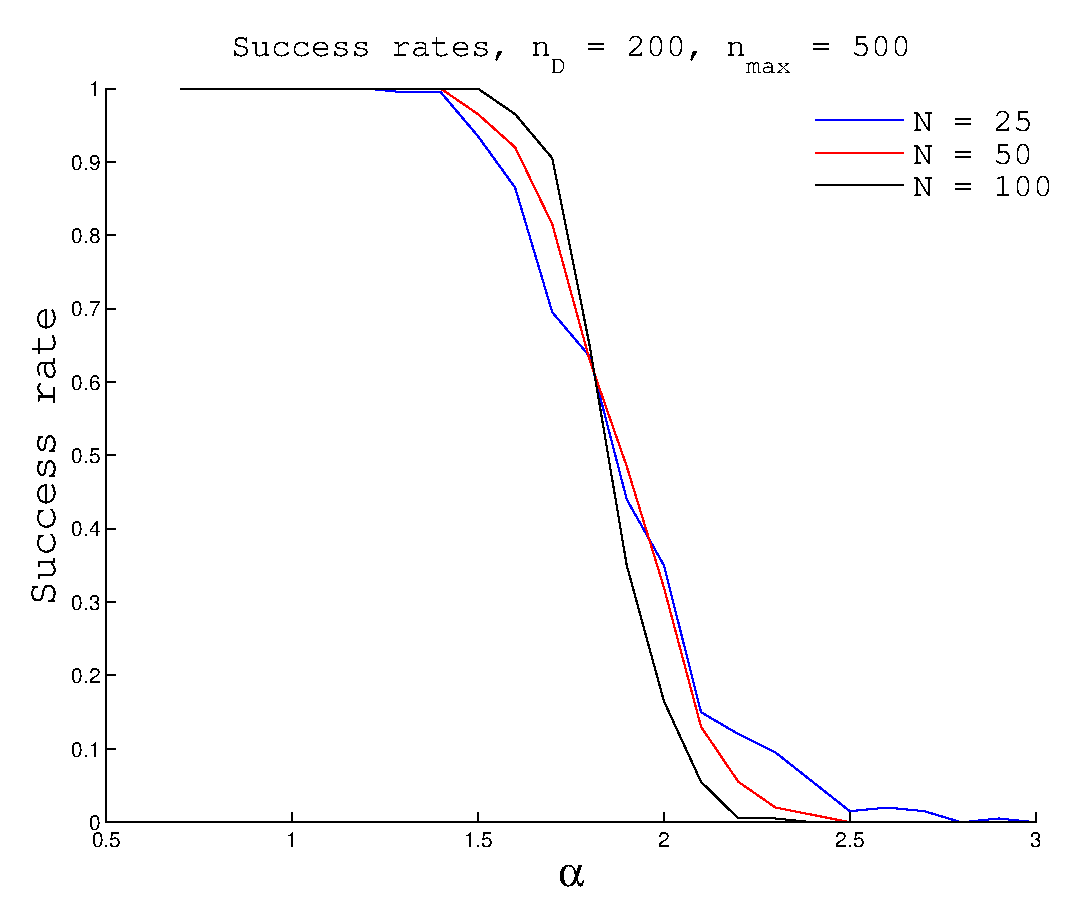
\includegraphics[width=\columnwidth]{success_rates_N_25_50_100_nd_200_nmax_500.eps}%
	\figcaption{Observed success rates.}
	\label{fig:observed_rates}
}
\myfigure{
	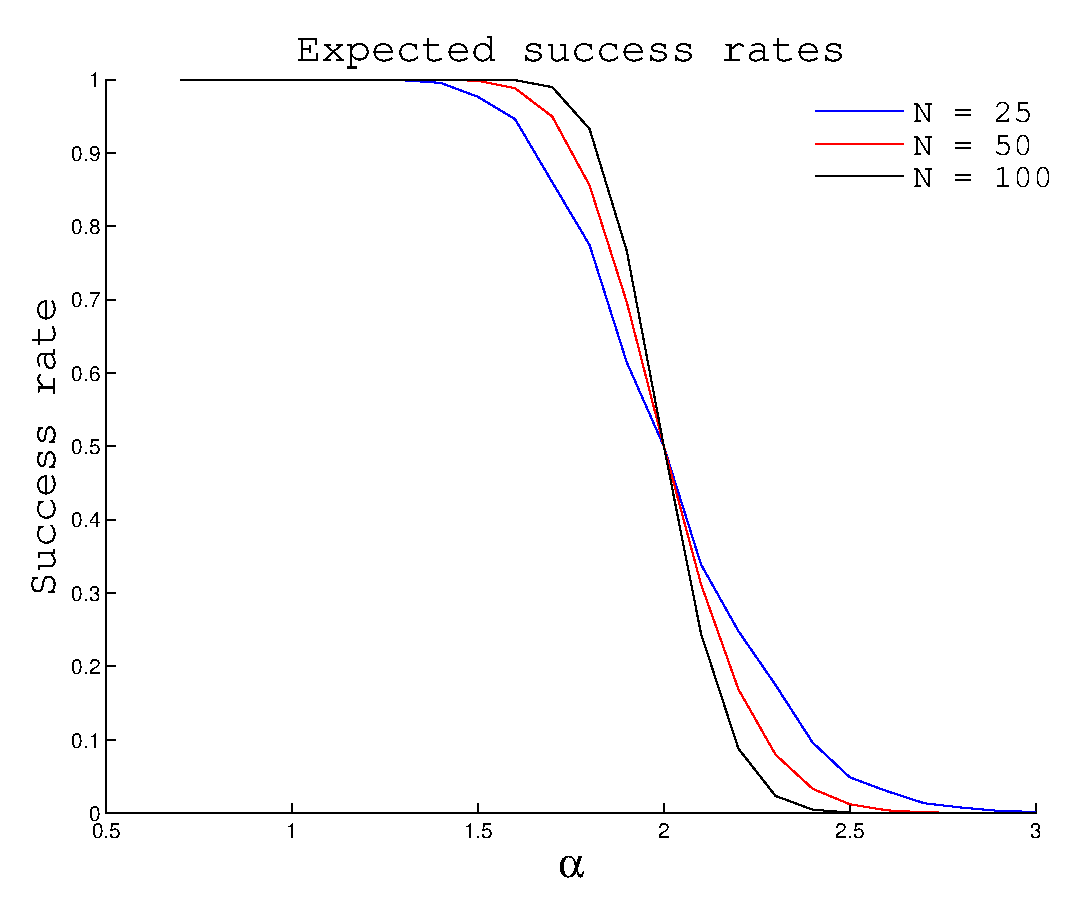
\includegraphics[width=\columnwidth]{expected_success_rates_N_25_50_100.eps}%
	\figcaption{Expected success rates.}
	\label{fig:expected_rates}
}

Extrapolating the trend to \(N=\infty\), it is expected that the success rate will be the step function.
That is:
\begin{equation} \label{eq:step}
	Q(\alpha) =
	\begin{cases}
	    1 & \alpha < 2\\
	    0 & \alpha > 2\text{.}
	\end{cases}
\end{equation}

All observed success rates are lower than the expected success rates.
This means that some datasets which were linearly seperable, have not been succesfully separated.
This makes sense, since only \(n_{max}\) sweeps are performed before giving up on finding a succesful weight vector.
Although the Rosenblatt algorithm is proven to converge in a finite number of steps, that doesn't mean it will converge fast; finite numbers can be large too.